\documentclass[border=3pt,tikz]{standalone}
\usepackage[utf8]{vietnam}
\usetikzlibrary{calc,angles,intersections,shapes.geometric,arrows,decorations.markings,arrows.meta,patterns.meta,patterns,quotes}
\usetikzlibrary{hobby}
\usepackage{tikz-3dplot,pgfplots}
\pgfplotsset{compat=1.15}
\usepgfplotslibrary{polar}
\usepackage{tkz-tab}
\usepackage{amsmath}
\usepackage[table]{xcolor}
\definecolor{darkblue}{HTML}{03346E}
\definecolor{dnvang}{HTML}{BB671B}%994D1C
\definecolor{dnxanh}{HTML}{0766AD}
\definecolor{dnxanhdam}{HTML}{19376D}
\definecolor{xanhngoc}{HTML}{116D6E}
\definecolor{dndo}{HTML}{BB2649}
\definecolor{dntrang}{HTML}{FFFFFF}
\def\mycolor{dnvang}
\def\mauphu{dnxanh}
\def\maudam{dnxanhdam}
\def\maunhan{dndo}
\def\mauchinh{darkblue}
\def\mautuongdong{xanhngoc}
\def\maunen{dntrang}
\begin{document}
	\newcommand{\electron}{\tikz \shade[ball color=\maudam] circle (0.4mm);}
	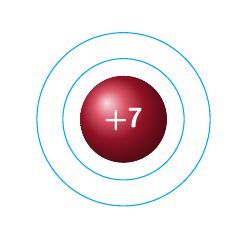
\begin{tikzpicture}[line cap=round,line join=round,declare function={r=0.55cm;}]
		\path (0,0) coordinate (O);
		\fill[ball color=\maunhan!70!red] (O) circle (r);
		\path (O) node [font=\bfseries\sffamily,color=white] (DTHN)  {+7};
		\draw [color=cyan] (O) circle (1.4*r)  (O) circle (2*r);
		\foreach \goc/\b in {90/1.4*r,-90/1.4*r,36/2*r,108/2*r,180/2*r,252/2*r,324/2*r}{
			\path (\goc:{\b}) [ball color=\maudam] node {\electron};
		}
	\end{tikzpicture}
\end{document}